% ============================================================
% Reporte: Factorial Recursivo en Ensamblador x86 (FPU)
% Autor: Edson Joel Carrera Avila
% ============================================================

\documentclass[12pt, letterpaper]{article}

\usepackage[utf8]{inputenc}
\usepackage[T1]{fontenc}
\usepackage[english]{babel}
\usepackage{geometry}
\usepackage{graphicx}
\usepackage{listings}
\usepackage{xcolor}
\usepackage{booktabs}
\usepackage{amsmath}
\usepackage{hyperref}
\usepackage{fancyhdr}
\usepackage{float}
\usepackage{caption}
\usepackage{tikz}
\usetikzlibrary{shapes.geometric, arrows.meta, positioning}

\geometry{top=2.5cm, bottom=2.5cm, left=3cm, right=2.5cm}

% --- Colores y estilo de código ---
\definecolor{codegray}{rgb}{0.95,0.95,0.95}
\definecolor{codegreen}{rgb}{0.0,0.5,0.0}
\definecolor{codeblue}{rgb}{0.0,0.0,0.65}
\definecolor{codepurple}{rgb}{0.45,0.0,0.55}

\lstdefinelanguage{MASM}{
    morekeywords={PROC,ENDP,END,PUSH,POP,MOV,ADD,SUB,CALL,RET,JMP,
                  JAE,FLD,FLD1,FCOMIP,FSUBP,FSTP,FMUL,DWORD,QWORD,PTR,EBP,ESP,ST},
    sensitive=false,
    morecomment=[l]{;}
}

\lstset{
    backgroundcolor=\color{codegray},
    basicstyle=\ttfamily\footnotesize,
    keywordstyle=\color{codeblue}\bfseries,
    commentstyle=\color{codegreen}\itshape,
    numbers=left, numberstyle=\tiny\color{gray}, numbersep=8pt,
    frame=single, rulecolor=\color{gray!50},
    breaklines=true, captionpos=b, tabsize=4,
    showstringspaces=false
}

\lstdefinestyle{cpp}{
    language=C++,
    backgroundcolor=\color{codegray},
    basicstyle=\ttfamily\footnotesize,
    keywordstyle=\color{codeblue}\bfseries,
    commentstyle=\color{codegreen}\itshape,
    stringstyle=\color{codepurple},
    numbers=left, numberstyle=\tiny\color{gray}, numbersep=8pt,
    frame=single, rulecolor=\color{gray!50},
    breaklines=true, captionpos=b, tabsize=4,
    showstringspaces=false
}

% --- Encabezado ---
\pagestyle{fancy}
\fancyhf{}
\rhead{Práctica 03 --- Factorial Recursivo en ASM}
\lhead{\textit{Edson Joel Carrera Avila}}
\cfoot{\thepage}
\renewcommand{\headrulewidth}{0.5pt}

% ============================================================
\begin{document}

% --- Portada ---
\begin{titlepage}
    \centering
    \vspace*{1.5cm}

    {\Large \textbf{Universidad Autónoma de la Ciudad de México}}\\[0.3cm]
    {\large Licenciatura en Ingeniería de Software}\\[0.2cm]
    {\large Arquitectura de computadoras}\\[2.5cm]

    \rule{\linewidth}{0.5pt}\\[0.4cm]
    {\LARGE \bfseries Práctica 03}\\[0.3cm]
    {\Large Factorial Recursivo en Ensamblador x86}\\[0.3cm]
    \rule{\linewidth}{0.5pt}\\[2cm]

    \begin{flushleft}
        \textbf{Alumno:} Edson Joel Carrera Avila \\[0.3cm]
        \textbf{Grupo:} 302 \\[0.3cm]
        \textbf{Profesor:} Prof. Mtro. Omar Nieto Crisóstomo \\[0.3cm]
        \textbf{Fecha:} \today
    \end{flushleft}
    \vfill
\end{titlepage}

\tableofcontents
\newpage

% ============================================================
\section{Introducción}

Esta practica consiste en calcular el \textbf{factorial} de un numero usando dos lenguajes al mismo tiempo: \textbf{C++} (entrada y salida de datos) y \textbf{ensamblador x86} (operación matemática). La idea es ver como un programa de alto nivel puede delegar trabajo a código ensamblador, que esta mas cerca del hardware.

El factorial de un numero es multiplicar ese número por todos los enteros positivos menores que el. Por ejemplo:

\begin{equation}
    5! = 5 \times 4 \times 3 \times 2 \times 1 = 120
\end{equation}

Matematicamente, se puede definir de forma \textbf{recursiva} (es decir, usando la misma operación pero con un valor mas pequeno cada vez):

\begin{equation}
    x! =
    \begin{cases}
        1               & \text{si } x \leq 1 \quad \text{(caso base)} \\
        x \cdot (x-1)! & \text{si } x > 1 \quad \text{(paso recursivo)}
    \end{cases}
\end{equation}

% ============================================================
\section{Organización del programa}

El proyecto tiene dos archivos que trabajan juntos:

\begin{table}[H]
    \centering
    \caption{Archivos del proyecto}
    \begin{tabular}{@{}lp{9cm}@{}}
        \toprule
        \textbf{Archivo} & \textbf{Que hace} \\
        \midrule
        \texttt{main.cpp}      & Le pide un número al usuario, llama a la función ensambladora y muestra el resultado. \\
        \texttt{Factorial.asm} & Contiene el calculo del factorial escrito en ensamblador. \\
        \bottomrule
    \end{tabular}
\end{table}

El flujo del programa es sencillo:

\begin{enumerate}
    \item El usuario escribe un número en la consola.
    \item C++ recibe ese número y lo pasa a la función ensambladora.
    \item La función ensambladora calcula el factorial de forma recursiva.
    \item C++ toma el resultado y lo imprime en pantalla.
\end{enumerate}

% ============================================================
\section{Código fuente}

\subsection{Programa principal (main.cpp)}

El código en C++ hace tres cosas: declarar que la función \texttt{Mi\_fact} existe en otro archivo, pedirle un numero al usuario, y mostrar el resultado.

\begin{lstlisting}[style=cpp, caption={main.cpp}]
#include <iostream>
using namespace std;

// Le decimos a C++ que esta funcion esta definida en el archivo .asm
extern "C" double Mi_fact(double x);

int main() {
    double numero;
    cout << "--- Calculadora de Factorial (ASM Recursivo) ---" << endl;
    cout << "Introduce un numero: ";
    cin >> numero;

    double resultado = Mi_fact(numero);
    cout << "El factorial de " << numero
         << " es: " << resultado << endl;
    return 0;
}
\end{lstlisting}

La linea \textbf{extern "C"} es el puente entre C++ y ASM. Le dice al compilador que no modifique el nombre de la función al momento de compilar, para que ambos archivos puedan encontrarse.

\subsection{Función ensambladora (factorial.asm)}

Aqui esta el nucleo del programa. La función recibe \texttt{x}, comprueba si es 1 o menos (caso base), y si no, se llama a si misma con \texttt{x - 1} y multiplica el resultado por \texttt{x}.

\begin{lstlisting}[language=MASM, caption={Factorial.asm}]
.586
.model flat, c

.code

Mi_fact PROC

    ; Preparar el espacio en memoria para trabajar
    PUSH    EBP
    MOV     EBP, ESP
    SUB     ESP, 8

    FLD     QWORD PTR [EBP+8]     ; Cargar el valor x

    ; Comparar x con 1.0
    FLD1                           ; Cargar 1.0
    FCOMIP  ST(0), ST(1)           ; Comparar: 1.0 >= x?
    JAE     es_caso_base           ; Si x <= 1, ir al caso base

    ; x > 1: calcular x * factorial(x - 1)
    FLD1
    FSUBP   ST(1), ST(0)           ; Calcular x - 1
    FSTP    QWORD PTR [EBP-8]      ; Guardar x - 1 temporalmente

    PUSH    DWORD PTR [EBP-4]
    PUSH    DWORD PTR [EBP-8]
    CALL    Mi_fact                ; Llamarse a si misma con (x - 1)
    ADD     ESP, 8

    FMUL    QWORD PTR [EBP+8]      ; Multiplicar resultado por x
    JMP     fin

es_caso_base:
    FSTP    ST(0)                  ; Descartar x
    FLD1                           ; Retornar 1.0

fin:
    MOV     ESP, EBP
    POP     EBP
    RET

Mi_fact ENDP
END
\end{lstlisting}

% ============================================================
\section{Como funciona la recursión}

Cada vez que la función se llama a si misma, guarda su estado actual en la \textbf{pila de memoria} resuelve el subproblema mas pequeño, y al regresar retoma donde se quedo.

Para \texttt{Mi\_fact(4.0)}, la cadena de llamadas es:

\begin{figure}[H]
    \centering
    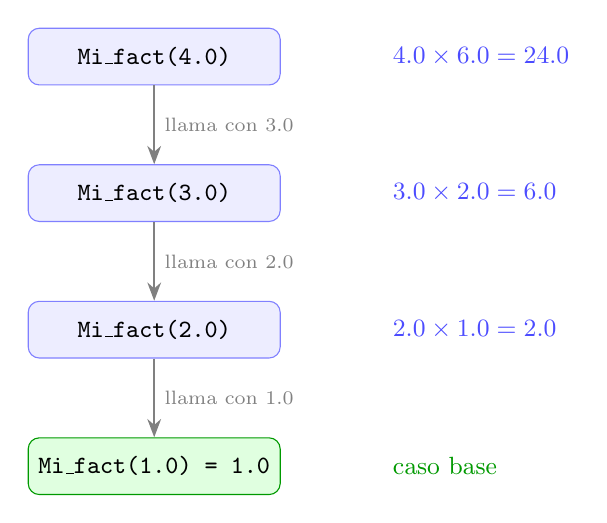
\begin{tikzpicture}[
        call/.style={rectangle, rounded corners, draw=blue!50, fill=blue!7,
                     minimum width=3.2cm, minimum height=0.72cm,
                     font=\ttfamily\small},
        base/.style={rectangle, rounded corners, draw=green!60!black, fill=green!12,
                     minimum width=3.2cm, minimum height=0.72cm,
                     font=\ttfamily\small},
        arr/.style={-Stealth, gray, thick}
    ]
        \node[call] (n4) {Mi\_fact(4.0)};
        \node[call, below=1cm of n4] (n3) {Mi\_fact(3.0)};
        \node[call, below=1cm of n3] (n2) {Mi\_fact(2.0)};
        \node[base, below=1cm of n2] (n1) {Mi\_fact(1.0) = 1.0};

        \draw[arr] (n4) -- node[right, font=\scriptsize]{llama con 3.0} (n3);
        \draw[arr] (n3) -- node[right, font=\scriptsize]{llama con 2.0} (n2);
        \draw[arr] (n2) -- node[right, font=\scriptsize]{llama con 1.0} (n1);

        \node[right=1.3cm of n1, font=\small, green!60!black] {caso base};
        \node[right=1.3cm of n2, font=\small, blue!70] {$2.0 \times 1.0 = 2.0$};
        \node[right=1.3cm of n3, font=\small, blue!70] {$3.0 \times 2.0 = 6.0$};
        \node[right=1.3cm of n4, font=\small, blue!70] {$4.0 \times 6.0 = 24.0$};
    \end{tikzpicture}
    \caption{Cadena de llamadas recursivas para \texttt{Mi\_fact(4.0) = 24}}
\end{figure}

Cada nivel espera a que el nivel inferior termine, multiplica el resultado por su \texttt{x} y lo regresa al nivel superior.

\begin{figure}[hbtp]
    \centering
    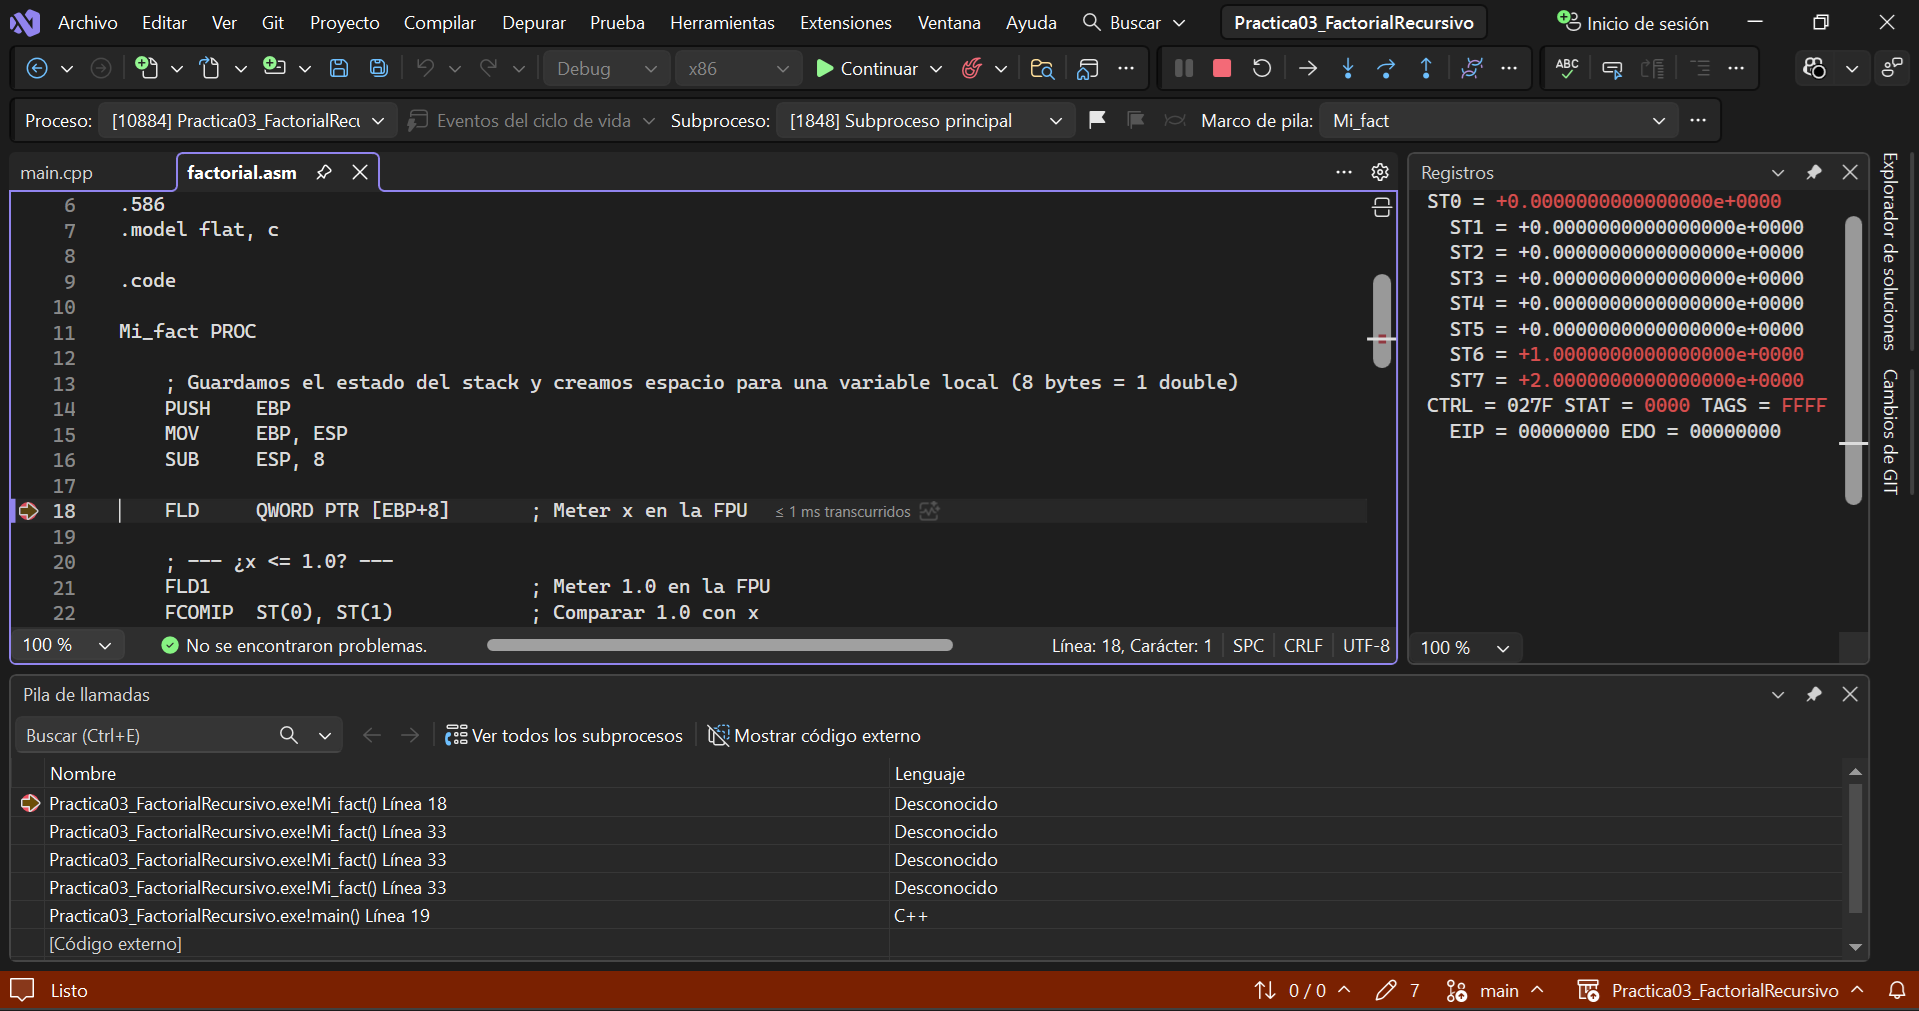
\includegraphics[width=1\textwidth]{call_stack.png}
    \caption{VS mostrando las llamadas apiladas de Mi\_fact.}
    \label{fig:etiqueta}
\end{figure}

% ============================================================
\section{La Unidad de Punto Flotante (FPU)}

El numero se maneja como \texttt{double} (numero con decimales de 64 bits) porque asi lo requiere la interfaz con C++. Para operar con este tipo de dato, el ensamblador usa la \textbf{FPU}, un componente del procesador dedicado a la aritmetica con decimales. La FPU tiene su propia pequeña pila interna de registros llamados \texttt{ST0} a \texttt{ST7}.

Las instrucciones FPU que usa esta practica son:

\begin{table}[H]
    \centering
    \caption{Instrucciones FPU utilizadas}
    \begin{tabular}{@{}lp{8.5cm}@{}}
        \toprule
        \textbf{Instrucción} & \textbf{Que hace en terminos simples} \\
        \midrule
        \texttt{FLD}    & Toma un numero de la memoria y lo coloca en la pila de la FPU. \\
        \texttt{FLD1}   & Coloca directamente el valor 1.0 en la pila FPU. \\
        \texttt{FCOMIP} & Compara dos numeros de la pila y le avisa al procesador cual es mayor. \\
        \texttt{FSUBP}  & Resta los dos numeros del tope de la pila FPU. \\
        \texttt{FSTP}   & Saca el numero del tope de la pila FPU y lo guarda en memoria. \\
        \texttt{FMUL}   & Multiplica el tope de la pila por un numero en memoria. \\
        \bottomrule
    \end{tabular}
\end{table}

\begin{figure}[hbtp]
    \centering
    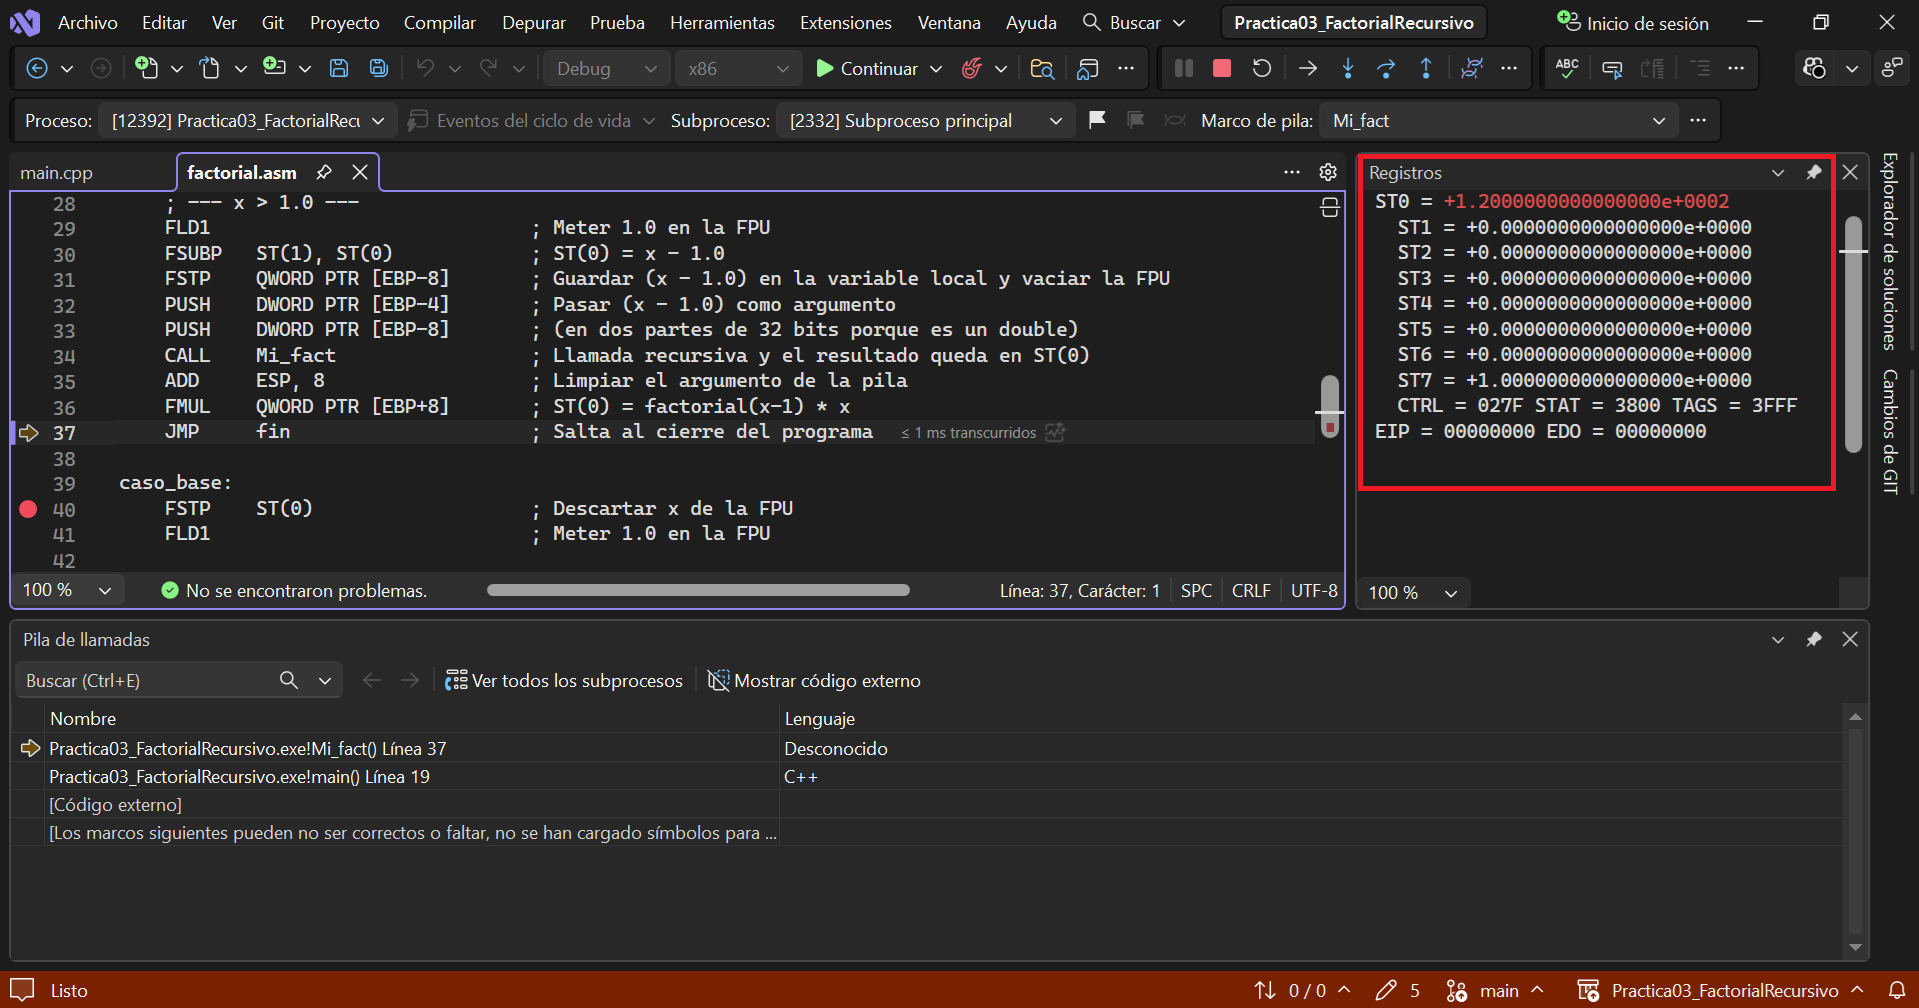
\includegraphics[width=0.7\textwidth]{registros.png}
    \caption{Ventana de registros con ST0-ST7 y sus valores númericos para 5!.}
    \label{fig:etiqueta}
\end{figure}

% ============================================================
\section{Ejemplo de ejecución}

Al correr el programa, la consola muestra:

\begin{verbatim}
--- Calculadora de Factorial (ASM Recursivo) ---
Introduce un numero: 6
El factorial de 6 es: 720
\end{verbatim}

\begin{figure}[hbtp]
    \centering
    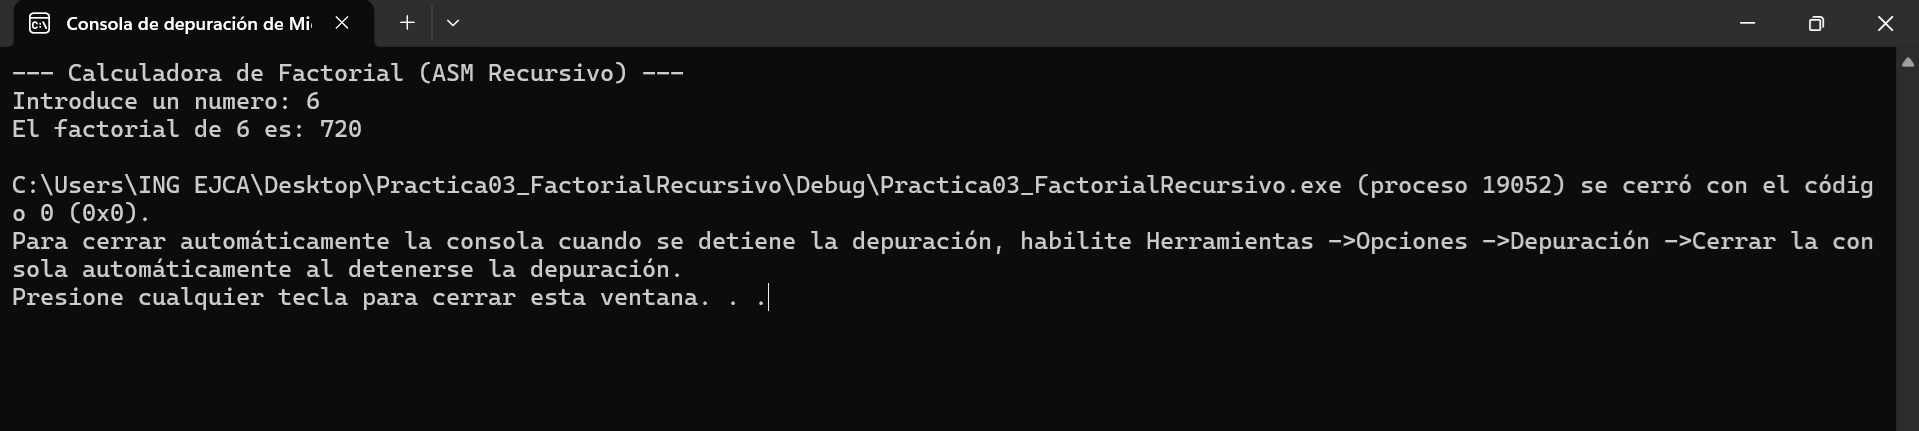
\includegraphics[width=1\textwidth]{consola.png}
    \caption{Vista de la consola, donde el usuario interactua.}
    \label{fig:etiqueta}
\end{figure}

% ============================================================
\section{Repositorio GitHub}

https://github.com/7mo-ArquitecturaComputadoras/Practica03\_FactorialRecursivo

% ============================================================
\section{Conclusiones}

\begin{itemize}
    \item Fue posible combinar C++ con ensamblador de forma sencilla gracias a \texttt{extern "C"}, que actua como puente entre los dos lenguajes.
    \item La recursión en ensamblador funciona igual que en cualquier lenguaje de alto nivel: cada llamada guarda su estado, espera el resultado del nivel inferior y continua. La diferencia es que en ensamblador todo ese manejo se hace instrucción por instrucción, de forma manual.
    \item El uso de la FPU permite trabajar con numeros de 64 bits, lo que hace a la función compatible con el tipo \texttt{double} de C++.
    \item Esta practica ayuda a entender lo que realmente ocurre dentro del procesador cada vez que un programa llama a una función, algo que los lenguajes de alto nivel ocultan automaticamente.
\end{itemize}

\end{document}

